% Chapter 2
%Chapter 2: 3D Rectification ( on PrimeSense, KinectV2, and Prosilica )all of equations
%2.1 From Depth to Z-coordinate
%2.2 From Z to X/Y
%2.3 3D Reconstructions for PrimeSense, KinectV2, and Prosilica
%Chapter 2: Camera Calibration Model(Compare pinhole camera  
%
%X= ExZ + Fx
%Y= EyZ + Fy
%with what we are doing)
\chapter{Real-Time 3D Rectification} % Main chapter title
\label{sens_Rectification} % For referencing the chapter elsewhere, use \ref{sens_Rectification} 
As analyzed in chapter \ref{sens_introduction}, traditional camera calibration based on pinhole camera model is not able to supply RGB-D cameras a satisfying real-time solution for lens and depth distortions. In this chapter, instead of using any models, a data based look-up table (LUT) method is used, which will not only suit for both of NearIR steams and RGB steams, but also for all of the universal RGB-D cameras. Rectifications of 3D world coordinates \(X^{w}\)/\(Y^{w}\)/\(Z^{w}\) will be separated into two parts. 
\\\\%
Above all, \(X^{w}\) and \(Y^{w}\) will be separately translated though two different transformation matrices that contains radial dominated lens distortions information. The transformation matrices are determined by pixels' coordinates-pairs ( image plan coordinates \(row\) / \(column\) and corresponding world coordinates \(X^{w}\)/\(Y^{w}\) ) that are extracted from captured uniform round dot grid pattern. Then, for each frame, external calibrated data from optical-flow sensor will be added as fixed \(Z^{w}\) for every pixel in the frame. After both of RGB stream and NearIR stream pixels find a match with world coordinate \(X^{w}\)/\(Y^{w}\)/\(Z^{w}\), depth data will be finally added for each pixel to generate a table of XYZWRGBD.

\section{\(X^{w}\)/\(Y^{w}\) Rectifications}
\label{sectionXY_rectification}
The uniform round grid captured by RGB/NearIR steams contains radial dominated distortions information, which will be used for \(X^{w}\)/\(Y^{w}\) rectifications, to generate transform matrices to translate image plane rows and columns to world coordinates \(X^{w}\)/\(Y^{w}\). In order to appropriately make use of the distortions information, the core mission is to locate the coordinates-pairs of each round dot. \\\\
%
The whole process of transformation matrices generation could be separated into three steps. %
The first step is to track the \((column, row)\) of each round dot cluster's center captured by RGB/NearIR steams, and the second step is to determine the corresponding world coordinates \((X^w, \,Y^w)\) for every \((column, row)\). After the coordinates-pairs are determined for every round dot cluster's center captured by RGB/NearIR steams, the last step is to use them to train high-order polynomial surface fitting models to generate transformation matrices, which could map from \((column, row)\) to \((X^w, \,Y^w)\) for every single pixel of a frame.
%
\subsection{Round Dot Center \((column, row)\) extraction}
\label{RowColumnExtraction}
The round dot pattern consists of black dots and white background. As the simplest way to segment black dots from background, which is not 100\% white in the captured image, thresholding (binarizing) is applied as pre-processing of the uniform grid's tracking, using Digital Image Processing (DIP) technologies. After an adaptive binarizing of a frame, a \enquote{sniffer} (edge modification) will be applied for captured clusters' centers determination, i.e., the extraction of (column, row) as clusters' centers.\par
%
\subsubsection{Digital Image Processings}
In this section, DIP technologies are used for the goal of RGB/NearIR steams' binarizing. Considering that the many steps of processing will be applied on every single pixel of every frame, using GPU (parallel processing) has more advantages on handling this kind of mission than using CPU. OpenGL is selected as image processing language, and the default data type of steams saved on GPU during processing will be Single-Floating type, with a range from 0 (balck) to 1 (white). For both of RGB steam and NearIR steam, steam data need to be saved onto GPU first, during which progress gray-scale converting is also done.\\%
\\\par%
 \qquad \textbf{Converting RGB/NearIR to Gray-Scale}\\%
In order to suit for both of the RGB and the NearIR steams, the first step of binarizing is to do gray-scaling. For NearIR steam, its data contains only color gray. There is no need to consider gray-scale problem, and data will be saved on GPU as single-floating automatically. Whereas for RGB steam, a conversion from RGB to gray value is needed. Typically, there are three converting methods: lightness, average, and luminosity. The luminosity method is finally chosen as a human-friendly way for gray-scaling, because it uses a weighted average value to account for human perception, which could be written as

\begin{equation}
%
Intensity_{\text{\_gray}} =  0.21 Red\,  + \, 0.72 Green \, + \, 0.07 Blue
%\label{lensDistortion}
%
\end{equation}%
%
\\\par%
 \qquad \textbf{Histogram Equalization}\\%
As values saved on GPU, all of the pixel intensity values are within the range of [0, 1], where \enquote{0} means 100\% black and \enquote{1}  means 100\% white. In practical, NearIR steam image is always very dark, as shown in figure \ref{Raw_Single_NIR} (with their intensity values every close to zero).  In order to enhance the contrast of NearIR image for a better binarizing, rescaling is necessary. In this section, histogram equalization technique is used maximize the range of valid pixel intensity distributions. Same process is also compatible on the RGB steam.\\\\
%
 \begin{figure}[h]
\hspace*{-0.5cm}
\centering
\subfloat[Raw NearIR][Raw]{
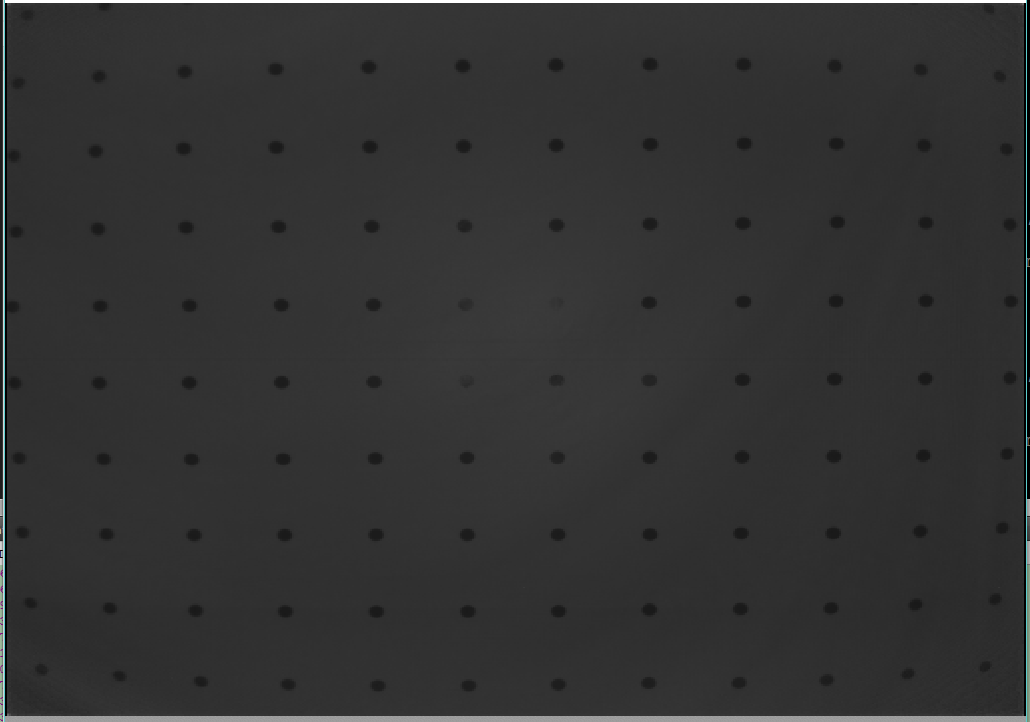
\includegraphics[width=0.5\textwidth]{Raw_Single_NIR}
\label{Raw_Single_NIR}}
\subfloat[Histogram Equalized NearIR][Histogram Equalized]{
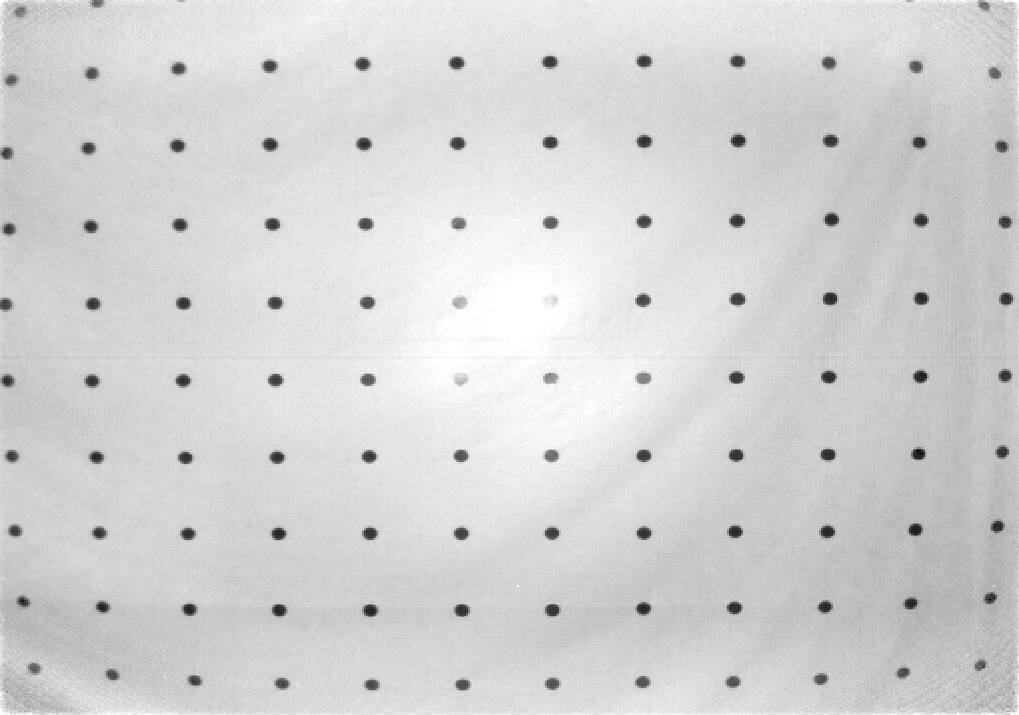
\includegraphics[width = 0.5\textwidth]{NIR_After_HistogramEqualization}
\label{NIR_After_HistogramEqualization}}
%\qquad
\caption{NearIR Streams before / after Histogram Equalization}
\label{Histogram_Equalization}
\end{figure}%
%
Commonly, Probability Mass Function (PMF) and Cumulative Distributive Function (CDF) will be calculated to determine the minimum valid intensity value (\(floor\)) and maximum valid value (\(ceiling\)) for rescaling, whereas tricks could be used by taking advantage of the GPU drawing properties.\\%
\\%
PMF means the frequency of every valid intensity value for all of the pixels in an image. Dividing all of the pixels in terms of their intensity values into \(N\) levels, every pixel belongs to one level of them, which is called gray level. With an proper selection of \(N\) to make sure a good accuracy, the intensity value of a pixel could be expressed based on its gray level \(n\), as\par%

\begin{equation}
%
Intensity = n/N * (1 - 0) + 0 = n/N
%\label{lensDistortion}
%
\end{equation}%
%
where \(n\) and \(N\) are integers and \(1 \leqslant n \leqslant N\).\\\\%
%
PMF calculation is very similar with the points-drawing process in terms of GPU that, both of them share the properties of pixel-by-pixel calculation. For the GPU points-drawing process onto a customer framebuffer, the single-floating \enquote{color} value could go beyond the normal range [0, 1], with a maximum value of a signed 32-bit integer (\(2^{31}\) - 1). And different \enquote{color} values will be added together to form a \enquote{summational-color} in the case that some pixels are drawn onto the same position coordinates. \textbf{Taking} the range of pixel intensity values [0, 1] \textbf{as} a segment on x-axis waiting to be drawn, the intensity frequency \textbf{as} the \enquote{summational-color} of multiple pixels with different intensity drawn at the same position, and the counting process of intensity frequency \textbf{as} a points-drawing process, PMF could be calculated by drawing all of the pixels onto the x-axis within the normal intensity range [0, 1], with every single pixel's position coordinates re-assigned as (\(pixel\_intensity\), \(0\)) and its \enquote{color} value constantly being equal to one. Given the width (range of x-axis) of customer framebuffer being [-1, 1] in OpenGL, which is twice the range of pixel intensity [0, 1], the half-width of the customer framebuffer is same with the total number \(N\) of gray levels, which determines the precision of \(floor\) / \(ceiling\) intensity selection. 
\\\\%
With PMF calculated and each intensity frequency that mapped to its corresponding gray level saved in the customer framebuffer, CDF could be easily calculated as
%
\begin{equation}
%
CDF(n) = \frac{sum}{N_{\text{\_Total Pixels/Image}}} 
%\label{lensDistortion}
%
\end{equation}%
%
where the gray level \(n\) is counted from the middle of the framebuffer's width to the end (1 \texttildelow \, \(N\)). And \(sum\) is the summation of customer framebuffer's values added up consecutively from 1 till \(n\).\\\\%
%
Then, at appropriate CDFs, e.g., \(CDF(n_{\text{\_floor}}) = 0.01\) and \(CDF(n_{\text{\_ceiling}}) = 0.99\), the intensities \(floor\) and \(ceiling\) could be written as
%
\begin{equation}
%
\begin{aligned}
floor &=  n_{\text{\_floor}} / N%
\\%
ceiling &=  n_{\text{\_ceiling}} / N
\end{aligned}
\label{intensityFloorCeilingDetermination}
%
\end{equation}%
%
Finally, a new intensity value of every single pixel in an image could be rescaled as
%
\begin{equation}
%
\begin{aligned}
Intensity_{\text{\_new}} &= \frac{Intensity_{\text{\_original}} - floor}{ceiling - floor} 
\end{aligned}
%
\end{equation}%
%
After this final rescaling step of Histogram Equalization, the new image gets better contrast effect, as shown in figure \ref{NIR_After_HistogramEqualization}%
\\\par%
 \qquad \textbf{Adaptive Thresholding}\\%
Affected by radial dominated lens distortions, the intensity value tend to decrease as the position of a pixel moves from the center of an image to the borders, in the case of observing a singular color view. Therefore, using fixed thresholding will generate too much noise around borders, and an adaptive thresholding process is needed. To segment the black dots from white background, we could simply subtract an image's background from an textured image. And an image's background comes from a blurring process on that image. \par%
%
 \begin{figure}[h]
\hspace*{-0.5cm}
\centering
\subfloat[Histogram Equalized NearIR][Histogram Equalized]{
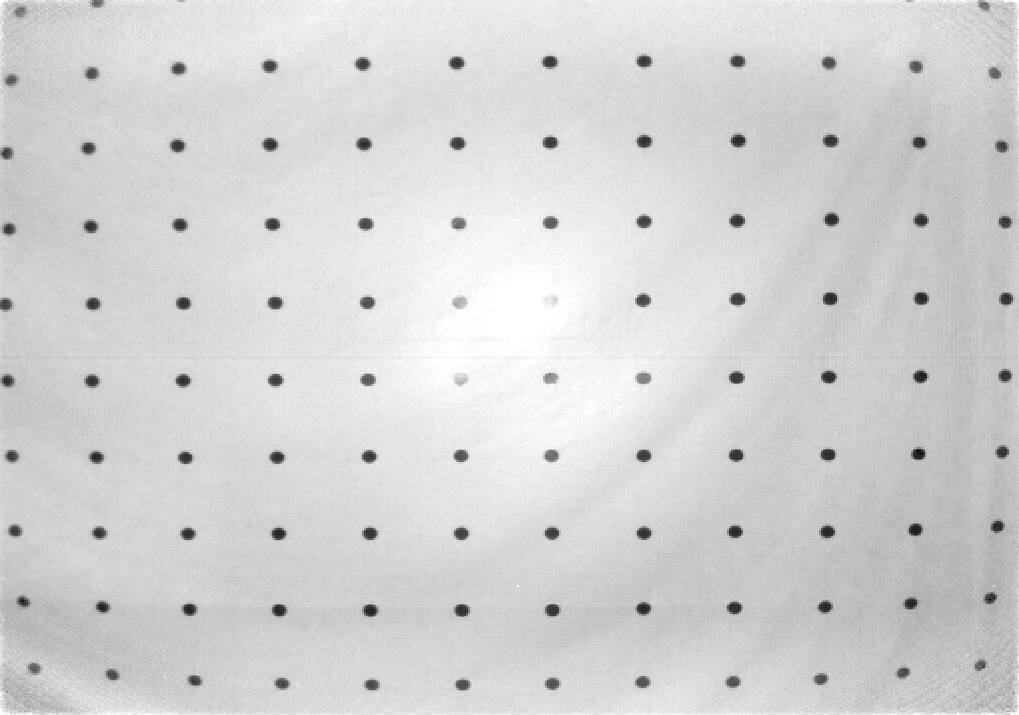
\includegraphics[width = 0.5\textwidth]{NIR_After_HistogramEqualization}
\label{NIR_After_HistogramEqualization}}
\subfloat[After Adaptive Thresholding][Binarized]{
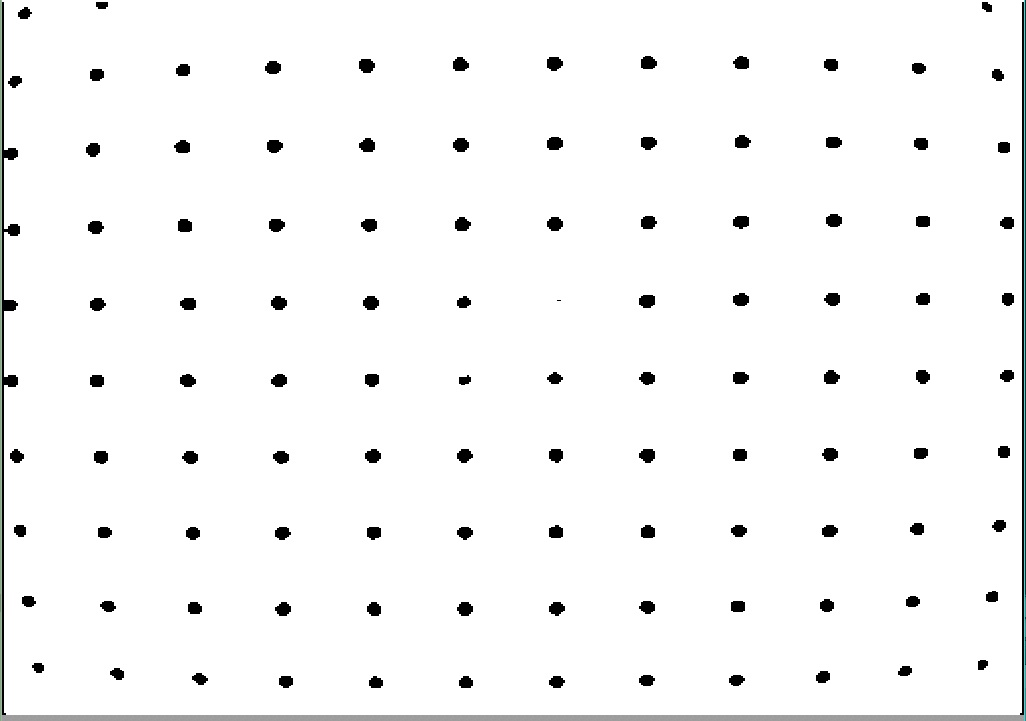
\includegraphics[width=0.5\textwidth]{Binarized_Single_NIR}
\label{Binarized_Single_NIR}}%\qquad
\caption{NearIR Streams before / after Adaptive Thresholding}
\label{Adaptive_Thresholding}
\end{figure}%
\par%
%
There are three common types of blurring filters: mean filter, weighted average filter, and gaussian filter. Mean filter is selected for this background-aimed blurring process, because it has the smallest calculation and also a better effect of averaging than the others. After the blurred image containing background information is obtained, the binarizing (subtraction) process for every single pixel could be written as

\begin{equation}
%
Intensity_{\text{\_binarized}} = %
%
\begin{cases}
\,\, 1 , \quad \quad I_{\text{\_textured}} - I_{\text{\_background}}  -  C_{\text{\_offset}} \,\, > \,\,0 %
\\%
\,\, 0 , \quad \quad \quad \quad else%
\end{cases}
%
\end{equation}%
%
where \(I\) is short for \(Intensity\) of every single pixel, and \(C_{\text{\_offset}}\) is a small constant that could be adjusted depending on various thresholding situations. In this project, \(C_{\text{\_offset}}\) is around 0.1.%
\\\\%
To sharpen the edge of the binarized image for a better \enquote{circle} shape detection, a median filter could be added as the last step of adaptive thresholding. As shown in figure \ref{Adaptive_Thresholding}, background is removed in the binarized image after adaptive thresholding.
%
%
\subsubsection{Sniffer for Round Dot Center}
After the adaptive thresholding, image data saved on GPU is now composed of circle-shaped \enquote{0}s within a background of \enquote{1}s. In order to locate the center of those \enquote{0}s circle, which is the center of captured round dot, it is necessary to know the edge of those circles. A trick is used to turn all of the edge data into markers that could lead a pathfinder to retrieve circle information.%
\\\\%
The idea that helps to mark edge data is to reassign pixels' values (intensity values) based on their surroundings. Using letter \(O\) to represent one single pixel in the center of a 3x3 pixels environment, and letters from \(A\)\texttildelow \(H\) to represent surroundings, a mask of 9 cells for pixel value reassignment could be expressed as below.

\begin{center}
  \begin{tabular}{ | c | c | c | }
    \hline
    \(E\) & \(A\) & \(F\) \\ \hline
    \(B\) & \(O\) & \(C\) \\ \hline
    \(G\) & \(D\) & \(H\) \\
    \hline
  \end{tabular}
\end{center}
%
To turn the surroundings \(A\)\texttildelow \(H\) into marks, different weights will be assigned to them. Those markers with different weights have to be non-zero data, and should be counted as the edge-part of circles. Therefore, the first step is to inverse the binary image, generating an image that consists of circle-shaped \enquote{1}s distributed in a background of \enquote{0}s.%
\\\\%
After reversing, the next step is to assign weight to the surroundings. OpenGL offers convenient automatic data type conversion, which means the intensity values from \enquote{0} to \enquote{1} of single-floating data type save on GPU could be retrieved to CPU as unsigned-byte data type from \enquote{0} to \enquote{255}. Considering a bitwise employment of markers, a binary calculation related weight assignment is used in the shader process for pixels. The intensity reassignment for every single pixel is expressed as the equation below.
%
\begin{equation}
\hspace*{-0.1cm}%
%
I_{\text{\_Path Marked}} = I_{\text{\_Original}} * \frac{(128I_{\text{A}} + 64I_{\text{B}} + 32I_{\text{C}} + 16I_{\text{D}} + 8I_{\text{E}} +  4I_{\text{F}} +  2I_{\text{G}}+I_{\text{H}})}{ 255 }
%
\label{snifferDistributionWeight}
\end{equation}%
\\%
After this reassignment, the image is not binary any more. Every non-zero intensity value contains marked information of its surroundings, data at the edge of circles are now turned into fractions. In other words, the image data saved on GPU at the moment is composed of \enquote{0}s as background and \enquote{non-zero}s circles, which contains fractions at the edge and \enquote{1}s in the center.%
\\\\%
Now, it is time to discover dots through an inspection over the whole path-marked image, row by row and pixel by pixel. Considering that, a process of one single pixel in this step may affect the processes of the other pixels (which cannot be a parallel processing), it is necessary to do it on CPU. The single-floating image data will be retrieved from GPU to a buffer on CPU as unsigned-byte data, waiting for inspection. And correspondingly the new CPU image will have its \enquote{non-zero}s circles composed of fractions at the edge and \enquote{1}s in the center. Whenever a non-zero value is traced, a dot-circle is discovered and a singular-dot analysis could start. The first non-zero pixel will be called as an anchor, which means the beginning of a singular-dot analysis. %
\\\\%
During the singular-dot analysis beginning from the anchor, very connected valid (non-zero) pixel will be a stop, and a \enquote{stops-address} queue buffer is used to save addresses of both visited pixels and the following pixels waiting to be visited. On very visit of a pixel, there is a checking procedure to find out valid (non-zero) or not. Once valid, the following two steps are waiting to go. The first step is to sniff, looking for possible non-zero pixels around as the following stops. And the second step is to colonize this pixel, concretely, changing the non-zero intensity value to zero. Every non-zero pixel might be checked 1\texttildelow 4 times, but will be used to sniff for only once.%
\\\\%
As for the sniffing step, base on the distribution table of \(A\)\texttildelow \(H\) that has been discussed above and their corresponding weight given by equation \ref{snifferDistributionWeight}, the markers \(A\)/\(B\)/\(C\)/\(D\) are valid (non-zero) as long as the intensity value of pixel \(O\) satisfies the following conditions shown as below.%
%
\begin{equation}
%
\begin{aligned}
if \,\, ( I_{\text{O}} \,\, \& \,\, \text{0x80}  == 1 ),\quad &then, \quad \text{marker } A\,\, \text{is valid \,\,( go Up )}%
\\%
if \,\, ( I_{\text{O}} \,\, \& \,\, \text{0x40}  == 1 ),\quad &then, \quad \text{marker } B\,\, \text{is valid \,\,( go  Left)}%
\\%
if \,\, ( I_{\text{O}} \,\, \& \,\, \text{0x20}  == 1 ),\quad &then, \quad \text{marker } C\,\,\text{is valid \,\,( go Right )}%
\\%
if \,\, ( I_{\text{O}} \,\, \& \,\, \text{0x10}  == 1 ),\quad &then,\quad \text{marker } D\,\,\text{is valid \,\,( go Down )}%
\\%
\end{aligned}
%
\end{equation}%
%
Once a valid marker is found, its address \((column, row)\) will be saved into the \enquote{stops-address} queue. One pixel's address might be saved for up to 4 times, but \enquote{colonizing} procedure will only happen once at the first time, so that the sniffing will stop once all of the connected valid pixels in a singular dot-cluster are colonized as zeros.%
\par%
%
 \begin{figure}[h]
\hspace*{-0.5cm}
\centering
\subfloat[After Adaptive Thresholding][before Extraction]{
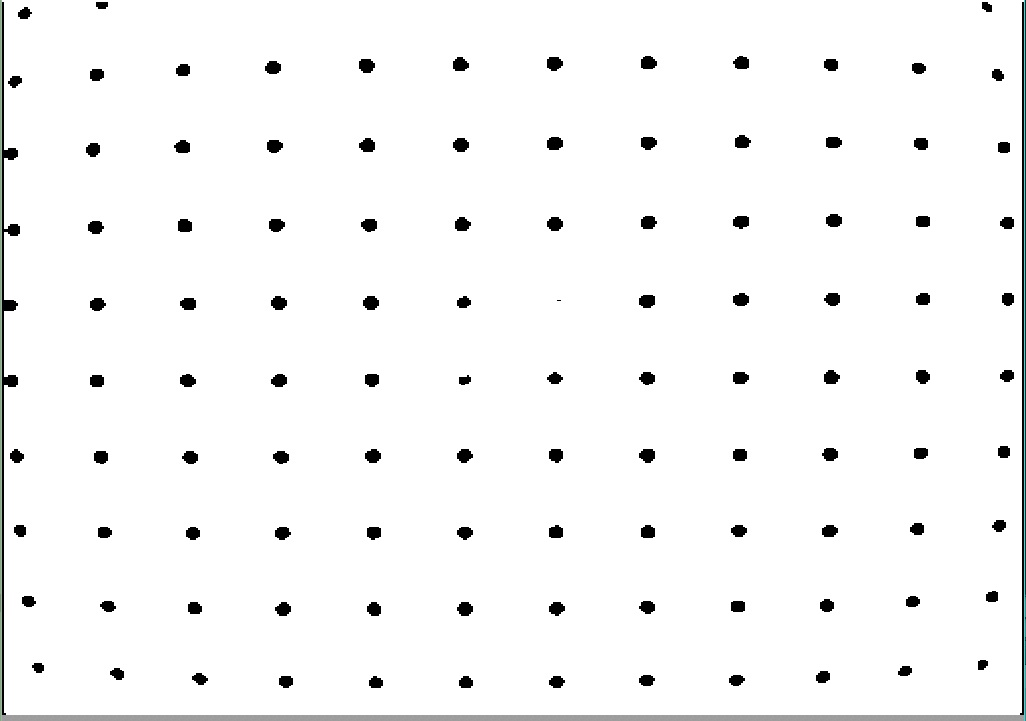
\includegraphics[width=0.5\textwidth]{Binarized_Single_NIR}
\label{Binarized_Single_NIR}}
%\qquad
\subfloat[Dot Centers Extraction][Extracted and Marked]{
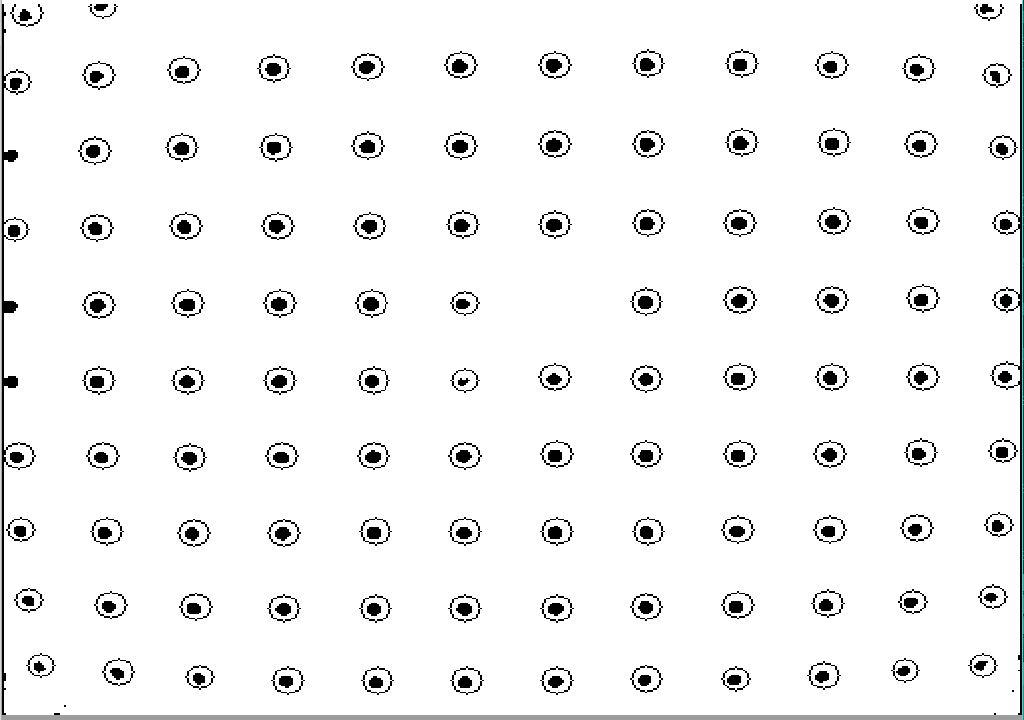
\includegraphics[width = 0.5\textwidth]{Dots_Extracted_Single_NIR}
\label{Dots_Extracted_Single_NIR}}
%
\caption{Valid Dot-Clusters Extracted in NearIR}
\label{DotCentersExtraction}
\end{figure}
%
In the second step \enquote{colonizing},  \(I_{\text{O}}\) is changed to zero, variable \(area\) of this dot-cluster pluses one, and bounding data \(RowMax\) / \(RoxMin\) / \(ColumnMax\) / \(ColumnMin\) are also updated.%
\\\\%%
Finally, the Round Dot Centers \((column, row)\) could be determined as the center of bounding boxes with their borders \(RowMax\) / \(RoxMin\) / \(ColumnMax\) / \(ColumnMin\). After potential noises being removed based on their corresponding \(area\) and shape (ratio of width and height), the data left are taken as valid dot-clusters. As shown in figure \ref{Dots_Extracted_Single_NIR}, the centers of valid dot-clusters are marked within their corresponding homocentric circles.
%
%
\subsection{\((X^w, \,Y^w)\) Fitting based on Uniform Grid}
\label{uniformGridFittingXY}
%
The list of round dot centers \((column, row)\)s is extracted through section \ref{RowColumnExtraction}. The following is to map every dot center's \((column, row)\) to its corresponding world coordinates \((X^w, \,Y^w)\). As shown in figure \ref{trackingModuleOnKinectV2CalibrationSystem}, world coordinates are from the uniform grid. Taking the side of unit-square (distance between two adjacent dots) as \enquote{Unit One} in the world coordinates and one dot as the origin of plan \(X^wY^w\), every dot cluster's center \(column\) / \(row\) will be mapped to integer values \(X^w\)/\(Y^w\). %
\\\\%
Ideally, a 3x3 perspective transformation matrix could help set a linear mapping between two plane coordinates, and 3 dot centers with know coordinates pair of \((column, row)\) and \((X^w, \,Y^w)\) are enough to determine the transformation matrix. Once four points with a squared-shape \(column\)/\(row\) distribution is found, a 3x3 perspective transformation matrix \(A\) could be determined by solving%
%
\begin{equation}
%
\left[ \begin{array}{c} %
zX^w \\ zY^w \\ z \end{array} \right] %
= %
A\cdot \left[ \begin{array}{c} %
C \\ R \\ 1 \end{array} \right] %
= %
\begin{bmatrix} 
a_{11} & a_{12} & a_{13} \\
a_{21} & a_{22} & a_{23} \\
a_{31} & a_{32} & a_{33} \\
\end{bmatrix}%
\cdot \left[ \begin{array}{c} %
C \\ R \\ 1 \end{array} \right] %
%
\end{equation}%
%
where \(C\) and \(R\) are vectors consist of \((column, row)\)s of four squared-shape distributed points; \(X^w\) and \(Y^w\) are vectors consist of four points \((0, 0)\), \((0, 1)\), \((1, 1)\), and \((1, 0)\); \(z\) denotes the third axis in the homogenous system connecting two planes. %
\\\\%
Due to the distortions, cluster centers in image plane are not uniformly distributed, and this 3x3 transformation matrix can only generate corresponding decimal \(X^w\)/\(Y^w\) values that are close integers. But in practical, the correct integer values \(X^w\)/\(Y^w\) could still be calculated through \(Rounding\). The list of cluster centers' image coordinate \((column, row)\)s can give many groups of four squared-shape distributed points, while each of them gives a different image coordinate distance that maps to the \enquote{Unit One} in world coordinates. Taking those points with generated \(X^w\)/\(Y^w\) values that are within an appropriate range close to integers as valid points, the \enquote{best} 3x3 transformation matrix could be determined by going through all of the possible groups of four squared-shape distributed points and picking out the group that leads to the most valid points.%
\\\\%
In this way, the so-called \enquote{best} transformation matrix can give a best \enquote{Unit One} distance in image coordinate, however its corresponding origin point \((0, 0)\), one of the four points that are used to calculate a transformation matrix, is usually not close to the center of cameras' Field of View (FoV). A translation matrix \(T\) could be used to refine the \enquote{best} transformation matrix, and help to translate the origin point to be a dot cluster that is closest to the center of FoV. The refined transformation matrix \(A_{\text{\_refined}}\) is written as%
%
\begin{equation}
%
A_{\text{\_refined}}%
= %
T \cdot A %
= %
\begin{bmatrix} 
1 & 0 & -X_{\text{\_Zero\_A}} \\%
0 & 1 & -Y_{\text{\_Zero\_A}} \\%
0 & 0 &   1 \\%
\end{bmatrix}%
\cdot A%
%
\end{equation}%
%
where the integer world coordinate point \((X_{\text{\_Zero\_A}}, \, Y_{\text{\_Zero\_A}})\) are mapped from the center point \((C_{\text{\_center}}, \, R_{\text{\_center}})\) of FoV in image plane by the so-called \enquote{best} transformation matrix \(A\), written as%
%
\begin{equation}
%
\left[ \begin{array}{c} %
zX_{\text{\_Zero\_A}} \\ zY_{\text{\_Zero\_A}} \\ z \end{array} \right] %
= %
A\cdot \left[ \begin{array}{c} %
C_{\text{\_center}} \\ R_{\text{\_center}} \\ 1 \end{array} \right] %
%
\end{equation}%
%
Eventually, the refined transformation matrix eventually generates a list of world coordinate points \((X^w, \, Y^w)\)s that correspond to image coordinates \((column, row)\)s. As shown in figure \ref{XY_GridFitting_Matlab}, world coordinates are integers and the origin (blue circle) is chosen as where the center-closest dot-cluster is sitting.\par%
%
 \begin{figure}[h]
\hspace*{-0.3cm}
\centering
\subfloat[Image Plane Coordinates][ImagePlane Coordinate]{
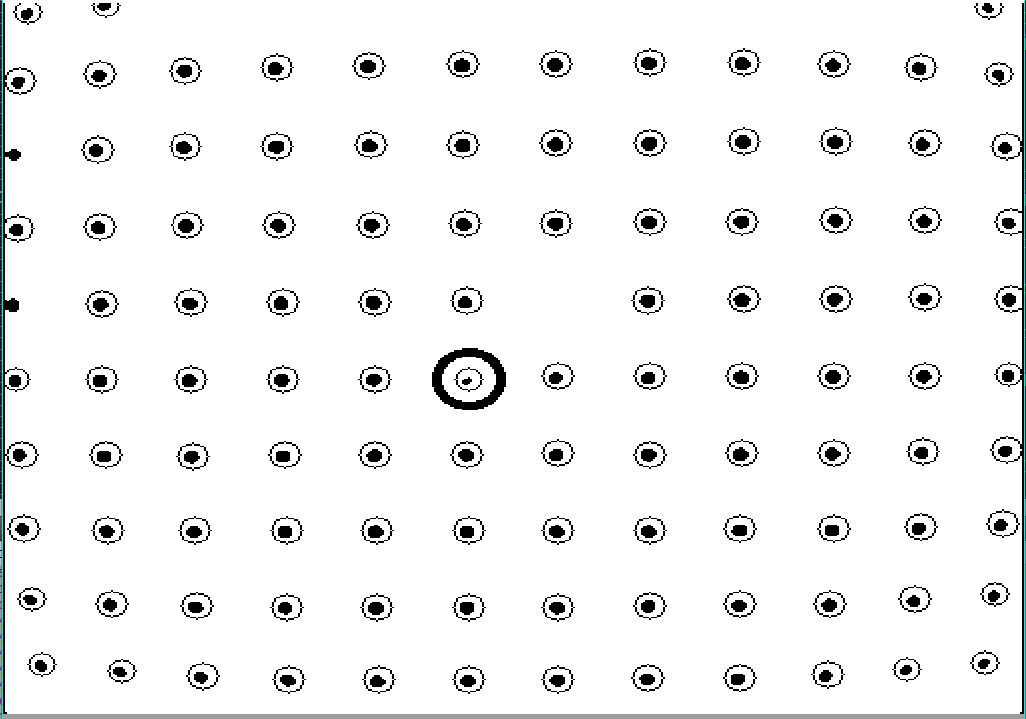
\includegraphics[width=0.54\textwidth]{Grid_Centered_Single_NIR}
\label{Grid_Centered_Single_NIR}}
%\qquad
\subfloat[World Coordinates][World Coordinate]{
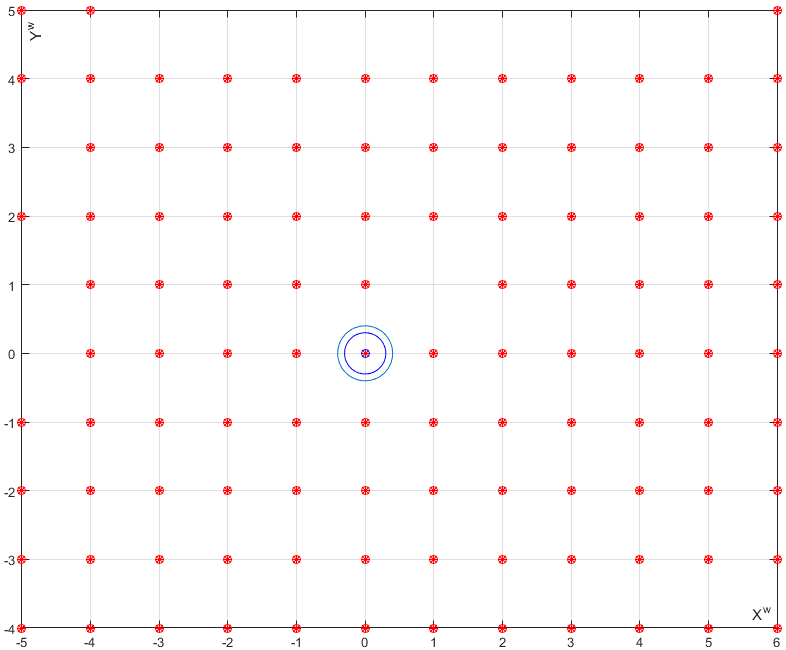
\includegraphics[width = 0.47\textwidth]{XY_GridFitting_Matlab}
\label{XY_GridFitting_Matlab}}
%
\caption{Coordinates-Pairs: (Row, Column)s and (\(X^w\), \(Y^w\))s}
\label{Grid_Fitting}
\end{figure}%
%
%
\subsection{High Order Polynomial Surface Mapping}
%
The 3x3 transformation matrix can only help to find the integer value list of  world coordinate \(X^w\)/\(Y^w\). It is not able to handle non-linear distorted mapping. Based on the lens distortion equation \ref{lensDistortion}, a higher order two-dimensional polynomial transformation matrix is needed for both of \(x\) and \(y\) rectification. Considering that the parameters in that equation, which means a surface mapping polynomial function, with power level larger than four are practically negligible, both of the second order and fourth order polynomial mapping are discussed below (prototyped in Matlab and realized in real-time image plane rectification).\\\\%
%
The second order polynomial mapping has 2x6=12 parameters, written as %
%
\begin{equation}
%
\begin{aligned}
X^w &=  a_{11}C^2 + a_{12}CR + a_{13}R^2 + a_{14}C + a_{15}R + a_{16}
\\%
Y^w &=  a_{21}C^2 + a_{22}CR + a_{23}R^2 + a_{24}C + a_{25}R + a_{26}
\end{aligned}
\label{secondOrderPolynomial}
%
\end{equation}%
%
similarly, the fourth order polynomial mapping has 2x15=30 parameters,\par%
%
\begin{equation}
%
\hspace*{-0.3cm}%
\begin{aligned}
X^w &=  a_{11}C^4 + a_{12}C^3R + a_{13}C^2R^2 + a_{14}CR^3 + a_{15}R^4 + a_{16}C^3 + a_{17}C^2R \\%
&\,\,\,\,\,\,+ a_{18}CR^2 + a_{19}R^3 + a_{110}C^2 + a_{111}CR + a_{112}R^2 + a_{113}C + a_{114}R + a_{115}
\\\\%
Y^w &=  a_{21}C^4 + a_{22}C^3R + a_{23}C^2R^2 + a_{24}CR^3 + a_{25}R^4 + a_{26}C^3 + a_{27}C^2R \\%
&\,\,\,\,\,\,+ a_{28}CR^2 + a_{29}R^3 + a_{210}C^2 + a_{211}CR + a_{212}R^2 + a_{213}C + a_{214}R + a_{215}
\end{aligned}
\label{fourthOrderPolynomial}
%
\end{equation}%
\\\par%
%
where \(C\) and \(R\) are shorted for \(Column\) and \(Row\).
\\\\%
To prototype equation \ref{secondOrderPolynomial} and \ref{fourthOrderPolynomial} in Matlab, \enquote{Curve Fitting Toolbox} is used to obtain the 2x6 and 2x15 parameters. Once those two set of parameters are obtained, the rectified image could also be determined, as shown in figure \ref{MatlabPrototpyeOfHighOrder},\par%
%
\begin{figure}[h]
\hspace*{-0.3cm}
\centering
\subfloat[\(2^{nd}\) Order][\(2^{nd}\) Order]{
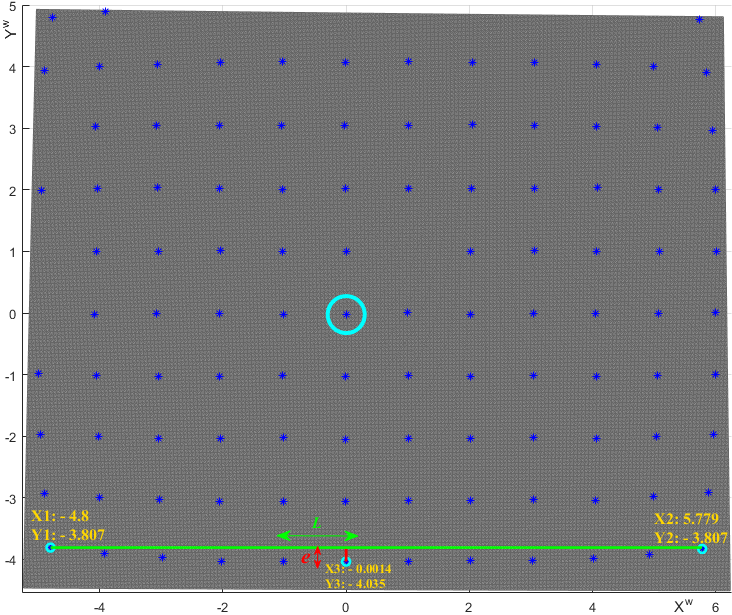
\includegraphics[width=0.5\textwidth]{Second_MatlabPrototype}
\label{Second_MatlabPrototype}}
%\qquad
\subfloat[\(4^{th}\) Order][\(4^{th}\) Order]{
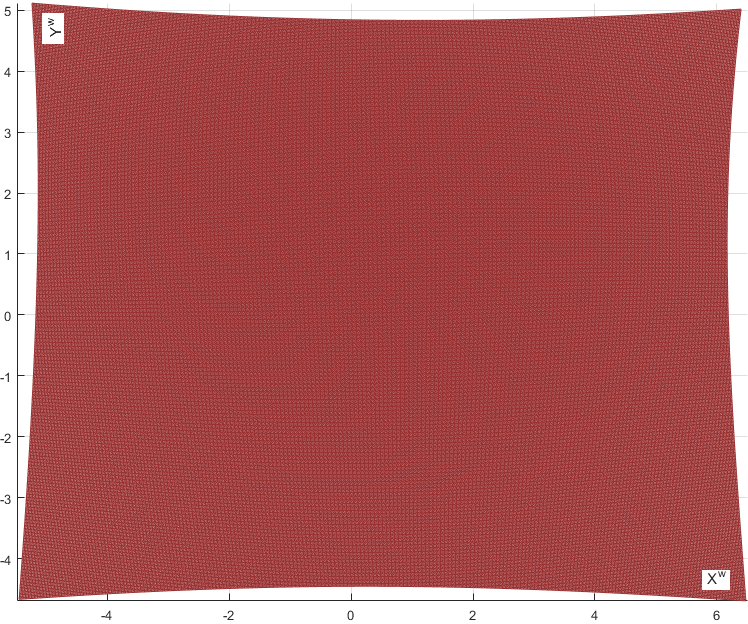
\includegraphics[width = 0.5\textwidth]{Fourth_MatlabPrototype}
\label{Fourth_MatlabPrototype}}
%
\caption{\(X^w\)/\(Y^w\) Matlab Prototype, \(2^{nd}\) / \(4^{th}\) Order Polynomial}
\label{MatlabPrototpyeOfHighOrder}
\end{figure}%
%
where based on \enquote{Goodness of fit} from Matlab, the Root-Mean-Square Error (RMSE) of (\(X^w\), \(Y^w\)) is (0.06796, 0.05638) for the \(2^{nd}\) order polynomial, and (0.02854, 0.02343) for the \(4^{th}\) order polynomial.
\\\\%
%
 \begin{figure}[h]
\centering
\subfloat[Before Rectification][Before Rectification]{
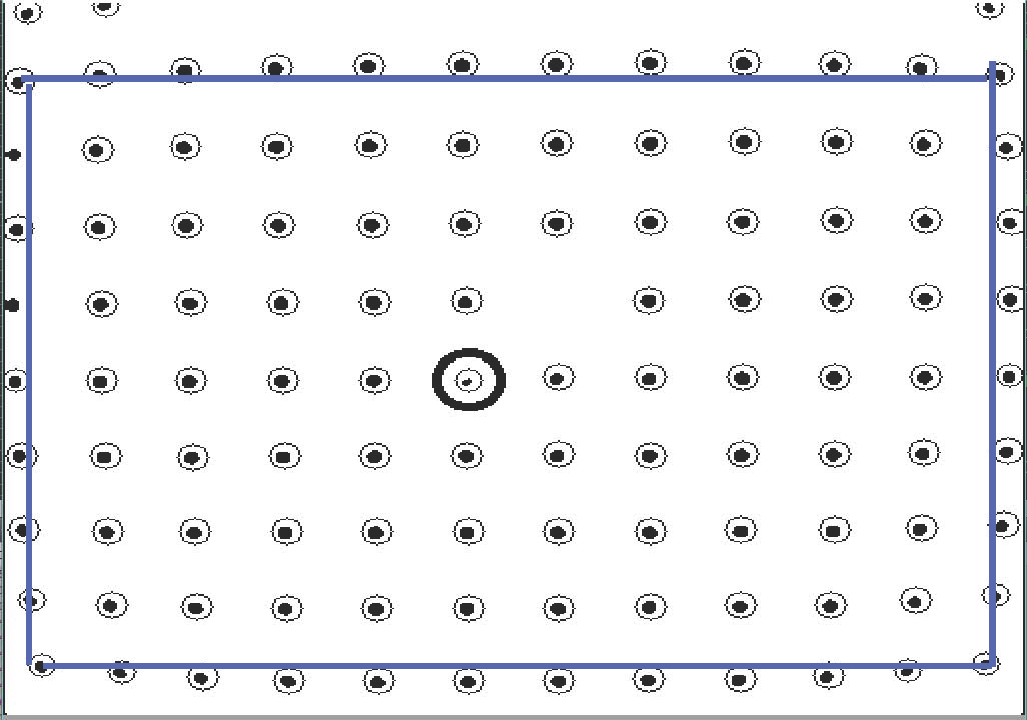
\includegraphics[height=0.42\textwidth, width=0.5\textwidth]{BeforeRectification_Single_NIR}
\label{BeforeRectification_Single_NIR}}
\\%\qquad
\hspace*{-0.3cm}
\subfloat[\(2^{nd}\) Order][\(2^{nd}\) Order]{
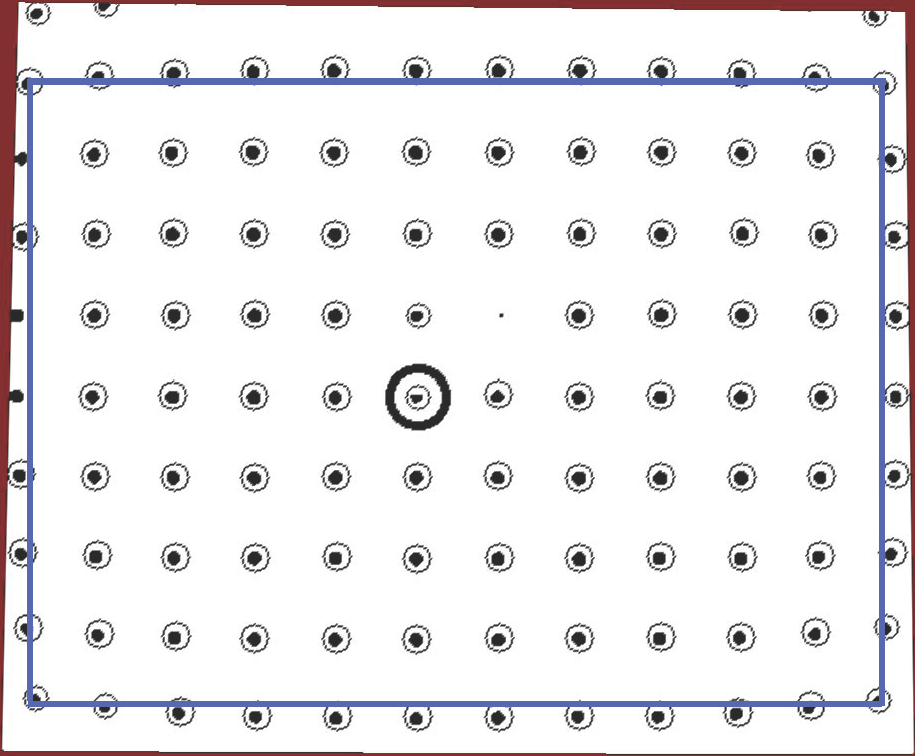
\includegraphics[width = 0.5\textwidth, height = 0.425\textwidth]{Second_QtScreenShot}
\label{Second_QtScreenShot}}
%
\subfloat[\(4^{th}\) Order][\(4^{th}\) Order]{
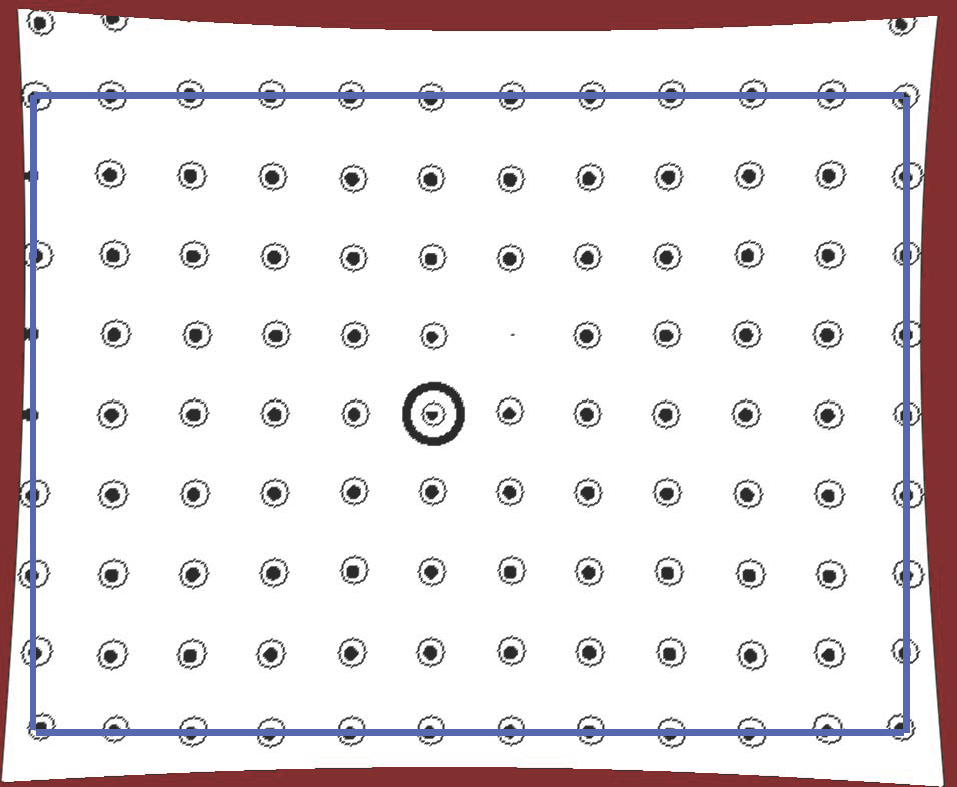
\includegraphics[width = 0.5\textwidth, height = 0.425\textwidth]{Fourth_QtScreenShot}
\label{Fourth_QtScreenShot}}
%
\caption{NearIR Stream High Order Polynomial Rectification}
\label{HighOrderNearIRRectification}
\end{figure}%
%
Then, apply those polynomial surface mappings into real-time steams rectification. We can see the rectified steam image from figure \ref{Second_QtScreenShot} and figure \ref{Fourth_QtScreenShot}, whose image-outline are same with Matlab prototypes, figure \ref{Second_MatlabPrototype} and figure \ref{Fourth_MatlabPrototype}. Gradually, from figure \ref{BeforeRectification_Single_NIR} to figure \ref{Fourth_QtScreenShot}, the dot-clusters on the outmost layer are more and more close to being sitting on the blue rectangle, which means less and less distortion.%
\\\\%
Not only from the comparison of RMSE, but more intuitively from figure \ref{HighOrderNearIRRectification}, we can tell that the \(4^{th}\) order polynomial surface mapping is much better than the second order. However, that more accurate process also cost more calculations, and requires more data (coordinate-pairs) to train the transformation model. Limited by the static dot pattern, fewer and fewer dot-clusters could be observed by the camera as the camera getting closer to the dot pattern. Practically, \(4^{th}\) order rectification is replaced by \(2^{nd}\) order when the number of dot-clusters is too few to train its transformation model.
%
%\subsection{Mathematical tools}
%\subsubsection{Singular Value Decomposition (SVD)}
%\subsubsection{Least Square with Pseudo-Inverse}
%
%
\section{\(Z^{w}\) Rectification}
%
Instead of from Depth steam, \(Z^{w}\) values will be determined directly from external real-world data. With the help of BLE Optical-Flow tracking module, as will be discussed later in section \ref{BLE_OF_TrackingModule}, \(Z^{w}\) values will be supported for every frame in real-time based on the camera's distance to the pattern. All of the pixels in one frame share the same \(Z^{w}\) in world coordinate.%
\\\\%
As well as the determination of \(X^{w}\)/\(Y^{w}\), which has been discussed in section \ref{uniformGridFittingXY},  \(Z^{w}\) value is also based on the uniform-grid's \enquote{Unit One},  the side of unit-square of the grid pattern. Concretely, the distance between every two adjacent dots' centers in real-world is 228mm. Therefore, \(Z^{w}\) = -\(|Z|\)(mm)/ 228(mm), where \(Z\) is the camera's working distance from the camera to dots pattern in reality offered by the BEL Optical-Flow tracking module. Choosing the origin to be where the camera is sitting, and the positives of \(X^{w}\)\(Y^{w}\) to be right and up, the \(Z^{w}\) values are always negative. Figure \ref{OneFrameXYZ_Rectified} shows one frame of 3D reconstruction in world coordinates based on rectified \(X^{w}\)/\(Y^{w}\) and \(Z^{w}\), where both of the origin and Z-axis are high-lighted as blue.%
%
\begin{figure}[h]
\centering
%rectified \(X^{w}\)/\(Y^{w}\) and \(Z^{w}\)
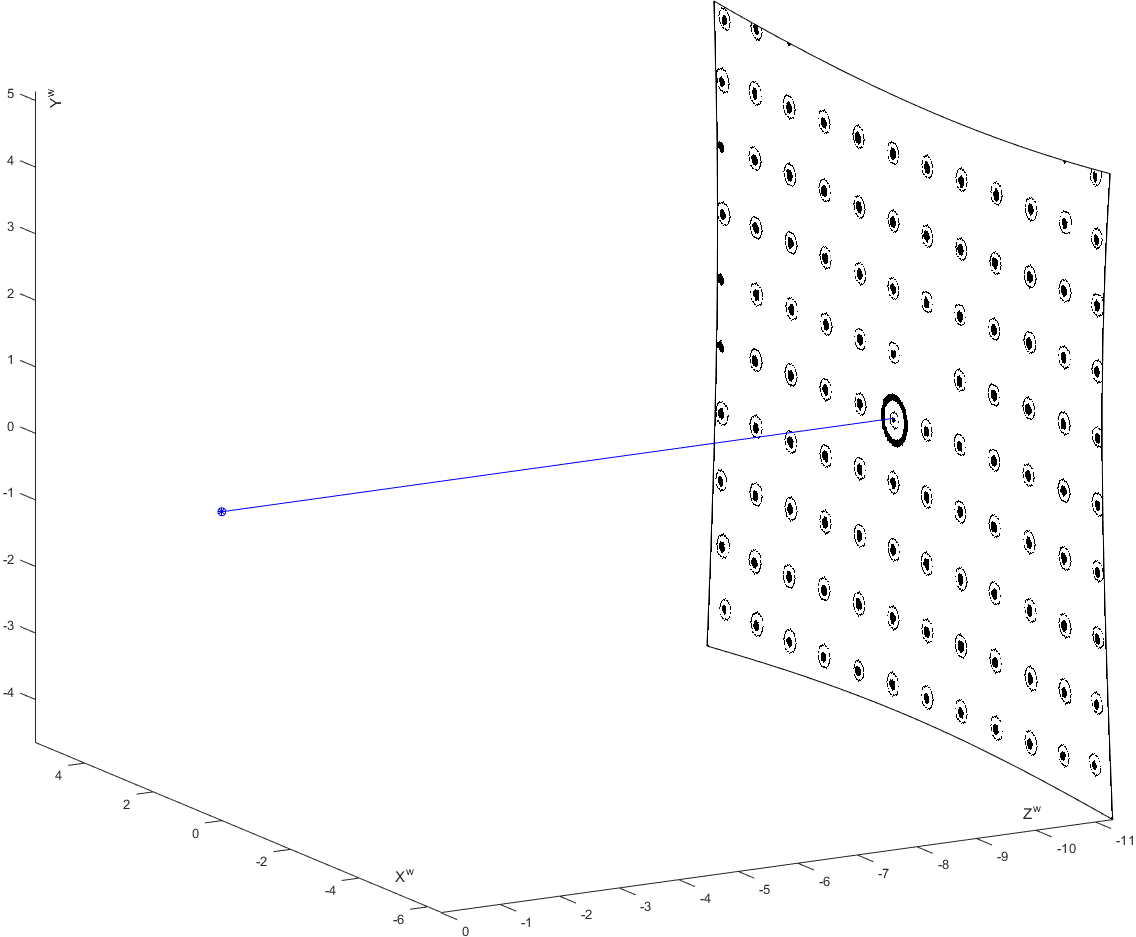
\includegraphics[width=0.7\textwidth, height= 0.5\textwidth]{OneFrameXYZ_Rectified}
\caption{NearIR Rectified \(X^{w}\)/\(Y^{w}\)/\(Z^{w}\) 3D Re-construction}
\label{OneFrameXYZ_Rectified}
\end{figure}%
%
\section{Data-Based XYZWRGB-D Look-Up Table}
In 3D re-construction, \(R\)/\(G\)/\(B\) and \(D\) (short for \(Depth\)) values are given for every pixel in one frame, while the rectified \(X\)/\(Y\)/\(Z\) (short for \(X^{w}\)/\(Y^{w}\)/\(Z^{w}\) in this section) values are determined by processes of looking up and calculating, which is based on \(D\). Therefore, the mission in this section is to find mappings from \(D\) to \(X\)/\(Y\)/\(Z\). Considering that, both of \(D\) and \(Z\) denote the distance from the camera to the object (dots pattern), it is straight forward to start from the relationship between \(D\) and \(Z\). As long as \(Z\) is obtained, \(X\) and \(Y\) for one single pixel could be determined through a linear relationship, due to the fact that the ray propagation is along a straight line.\\%
%
\begin{figure}[h]
\centering
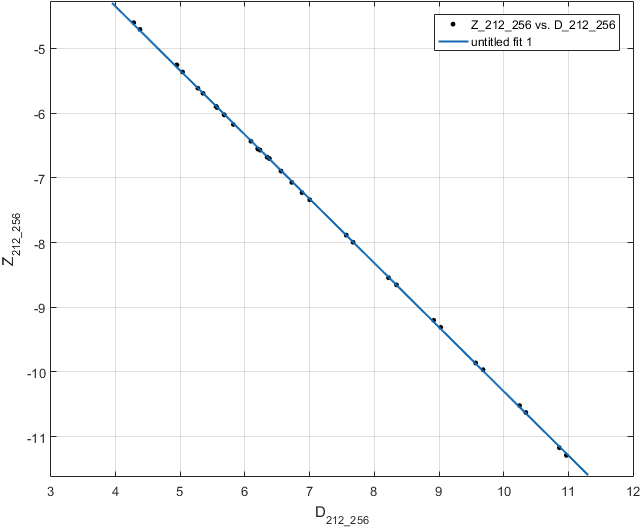
\includegraphics[width=0.8\textwidth]{ZD_CurveFitting}
\caption{Polynomial Fitting between D and Z}
\label{ZD_CurveFitting}
\end{figure}%
%
%%
%
\subsection{From \(D\) to \(Z\)}
%%
Both of \(D\) and \(Z\) are continuous data, so that their function could written as a polynomial expression, based on Taylor series. Figure \ref{ZD_CurveFitting} shows the polynomial fitting result, with 32 \(D\)/\(Z\) values (at pixel \(column\)=256 and \(row\)=212) from 32 frames, from Matlab \enquote{Curve Fitting Tool} toolbox. It is apparent that \(Z\) is linear with \(D\), which is also reasonable. Therefore, for every single pixel, \(Z\) could be retrieved from \(D\) through \par
%
\begin{equation}
Z(col, \, row) = a_{(col, row)}D(col, \, row)+b_{(col, row)}
\label{fromD_To_Z}
\end{equation}%
%
where \({(col, row)}\) denote the address of a pixels,  \(a_{(col, row)}\) and \(b_{(col, row)}\) are the corresponding linear coefficients that help map from \(D\) to \(Z\).%
%%
%
\subsection{From \(Z\) to \(X\)/\(Y\)}
For every possible \(Z\), within the slider's range on the rail, \(X\)/\(Y\) values for all of the pixels are rectified (as discussed in section \ref{sectionXY_rectification}). As for every single pixel, its view, a beam in 3D space, determines the linear relationships for both of \(Z\)-\(X\) and \(Z\)-\(Y\).
%
\begin{figure}[h]
\centering
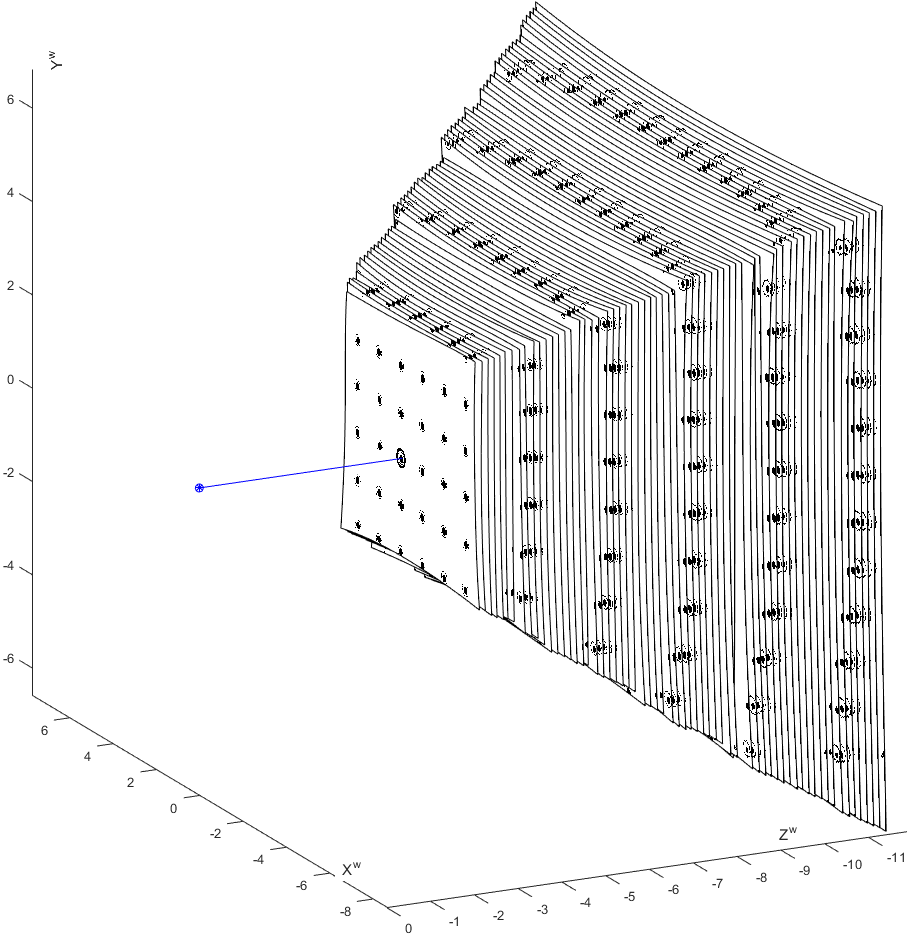
\includegraphics[width=0.7\textwidth, height= 0.55\textwidth]{Data63FranesForLUT}
\caption{63 Frames NearIR Rectified 3D Reconstruction}
\label{Data63FranesForLUT}
\end{figure}%
%
Figure \ref{Data63FranesForLUT} shows 63 frames of NearIR rectified 3D reconstruction, which gives an intuitionally pyramid shape of a camera sensor's field of view. The pyramid is composed of all of the pixel-beams, every single one of which could be expressed as \\%
%
\begin{equation}
%
\begin{aligned}
X(col, \, row) &= c_{(col, row)}Z(col, \, row)+d_{(col, row)}
\\%
Y(col, \, row) &= e_{(col, row)}Z(col, \, row)+f_{(col, row)}
\end{aligned}
\label{fromZ_To_XY}
%
\end{equation}%
%
where \({(col, row)}\) denote the address of a pixels, \(c\)/\(d\)/\(e\)/\(f\) are the corresponding linear coefficients that help map from \(Z\) to \(X\) and \(Y\).%
\\\\%
Figure \ref{SampleBeams_NearIR} shows some sample beams composed of coefficients \(c\)/\(d\)/\(e\)/\(f\), which gives a rectified field of view. It explains the lens distortions affections, that those beams are converged in front of the origin.\\%
%
\begin{figure}[h]
\centering
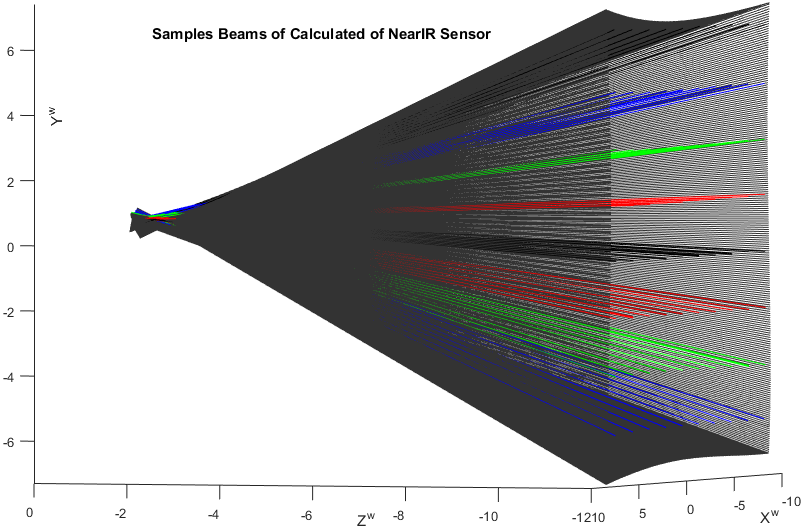
\includegraphics[width=0.77\textwidth]{SampleBeams_NearIR}
\caption{Sample Beams of Rectified NearIR Field of View}
\label{SampleBeams_NearIR}
\end{figure}%
\\%
To combine equation \ref{fromD_To_Z} and \ref{fromZ_To_XY}, a rectified 3D coordinate (\(X\), \(Y\), \(Z\)) for every single pixel could be looked up based on \(D\). With enough data generating a  \(column\)-by-\(row\)-by-\(6\)  look-up table that contains 6 coefficients (\(a\),\(b\),\(c\),\(d\),\(e\),\(f\)) for every single pixel, a rectified real-time 3D reconstruction could be displayed.
%
\section{Real-time analysis}
from Kai's SL based beam expansion to data based per-pixel beam in 3D space
%X= ExZ + Fx
%Y= EyZ + Fy

\section{3D Reconstruction differences for PrimeSense, KinectV2, and Prosilica}
shader comparison
%
%
%
%
%
%
%































